%%%%%%%%%%%%%%%%%%%%% chapter.tex %%%%%%%%%%%%%%%%%%%%%%%%%%%%%%%%%
%
% sample chapter
%
% Use this file as a template for your own input.
%
%%%%%%%%%%%%%%%%%%%%%%%% Springer-Verlag %%%%%%%%%%%%%%%%%%%%%%%%%%
%\motto{Use the template \emph{chapter.tex} to style the various elements of your chapter content.}

\chapter{Introduction}
\label{chap:Introduction}


\section{Fundamental Physics}
\label{intro:intro}

The scope of fundamental physics is to figure out an understanding in the form of models and/or theories of the base, the fundamental elements, from which everything else develops. That is precisely what Nuclear and subnuclear physics is about. As we will see in Chapter~\ref{Fundamentals-I}, the intuition that there are basic constituents of nature came quite early in ancient Greece almost three millennia ago, however it is really only in the XX century that a major leap in our understanding of nature at microscopic scales occurred. The turn of the century marked a major transition that brought remarkable theoretical and experimental developments which led to {\bf Modern Physics}.\\

Nuclear and Subnuclear physics is the  branch of Modern Physics and the field of study of the atomic nuclei as well as their constituents and their interactions. The fundamental extension of Subnuclear physics is the field of \emph{Particle Physics} which is related to the study of the fundamental components and forces of the Universe. Our current understanding of forces and constituents, apart of the Gravitational interaction, is enclosed in a single theory, known as the \emph{Standard Model} of particle physics. A complete description of the Standard Model is beyond the scope of these lectures, but it should be emphasised that Nuclear and Subnuclear physics are the foundations of Particle Physics and thus of its Standard Model (SM). In order to achieve a proper description of the SM, a significant background is needed both theoretical and experimental. The aim of these lectures is to give these fundamental elements. \\

The construction of our fundamental understanding of nature led to completely new concepts and the remarkable predictive power of the theoretical insights introduced have been able to predict the existence of phenomena that were observed only later. As we will see later in this Chapter, understanding the nature at small scales requires a higher resolution power in distance scales and therefore higher momenta of probe particles, which in turn requires a relativistic description of the systems. Also, microscopic scales make a Quantum Mechanical description unavoidable. The theoretical framework for the description of the phenomena in these lectures will require a solid bases in the two areas of modern physics and will start the construction of the common theoretical framework of relativistic Quantum Mechanics. This will lead to completely new concepts that have remarkable predictable consequences, such as the prediction of anti-matter which was predicted well before it was observed in nature. These lectures will cover the construction of our understanding of the nucleus, and the processes related to nuclear physics, such as the radioactive radiation ($\alpha$, $\beta$ and $\gamma$) and the bases of particle physics, with the rationale for the existence of {\it "hadrons"} and their decays as well as the existence of {\it "leptons"} which are heavy replicas of the electrons. The terms {\it "hadrons"} and {\it "leptons"} will be explained and correspond to specific particles that have specific roles in nature. \\

The scope of Nuclear and Subnuclear physics is not to be only descriptive of the building blocks of nature. Understanding their role in nature, the underlying reason for their existence and the fundamental laws that governs them is the wider scope. The introduction of {\it "hadrons"} is therefore done through their role in mediating the strong interaction, that is the necessary interaction to explain the existence of atomic nuclei. To get there however another major two new steps will need to be introduced. The first will be a description of short range forces through the first step into a relativistic Quantum Mechanical description of nature. The second will be on how interactions are not the result of {\it action at a distance}, but from the exchange of another type of particles: {\it "bosons"}. A concept that is natural in special relativity, but is a bit more involved to describe from the Quantum Mechanical point of view, but will done through time dependent perturbation theory and the introduction to Feynman diagrams. These bases will then lead to further theoretical developments in relativistic quantum mechanics, relativistic quantum field theory, gauge field theories and fundamental symmetries, which are outside the scope of these lectures. \\

Beside the significant theoretical developments, also remarkable experimental developments had to be achieved and require substantial introduction. \\

The Standard Model (SM) has been proven as a valid and coherent theory on the high energy (or small distance) scale, and this is the first time that such a thing happens in our history. The construction of the SM is the result of many experimental and theoretical efforts, made by mankind along centuries. \\

In order to achieve a proper understanding of this theory, a significant background is needed and these notes can be seen as a first introduction to \emph{Elementary Particle Physics} and \emph{Nuclear Physics} for a third year bachelor student, in order to get the needed preliminary knowledge to understand more advanced courses like:

\begin{itemize}
    \item Relativistic quantum mechanics
    \item Electroweak Interactions
    \item Quantum Field Theory
    \item Quantum Electrodynamics
    \item Fundamental Symmetries
    \item Particle Physics
    \end{itemize}
    
\section{An Extraordinary Convergence and Modern Microscopic Physics}

Modern physics, was really born with the Galillean and Newtonian theory of gravity, providing an incredibly successful and simple law that explained an unprecedented succession of phenomena at ever larger distant scales of observation from pendulums or the free fall of objects on earth to the motion of planets, stars, galaxies and clusters of galaxies, until small deviations required the modification and further insights of general relativity to complete this very precise and predictive picture. The event of Modern Physics at microscopic scales took longer and occurred through an extraordinary convergence of theoretical and experimental developments that lead to our understanding of the laws of nature at microscopic scales through Nuclear and Subnuclear physics, {\it viz.} the main scope of these lectures. \\

In a handful of decades, from the mid XVIIIth century to the beginning of the XIXth century an extraordinary convergence of theoretical and experimental physics discoveries have led to the birth of {\bf Modern Physics}:
\begin{enumerate}
\item the rise of Modern Atomism;
\item understanding the nature of light and birth of electromagnetism;
\item the theory of relativity;
\item the birth of Quantum Mechanics;
\item the discovery of radioactivity.
\end{enumerate}

All of these aspects but the last pertain to chemistry, analytical mechanics, electromagnetism and  quantum mechanics. This course will recap briefly in Chapter~\ref{Fundamentals-I} the rise of Modern Atomism, in Chapter~\ref{Relativity} special relativity. In Chapter~\ref{decaylaws-I} the principal elements of the discovery of radioactivity will be given. These are the fundamental elements to then discuss in more detail nuclear and subnuclear (or particles) physics. Various fundamental aspects of Quantum Mechanics will be reviewed in discussing scattering throughout the course.

    
\section{Role of Nuclear and Subnuclear Physics}    

Let's try to be a bit more specific on some of the points discussed in Section~\ref{intro:intro}. \\

Since in this course we'll be discussing various new theories, it is perhaps worth recalling the definition of {\it scientificity} as how we move from observations to {\it universal laws}! The formal definition by Karl Popper in his {\it "The Logic of Scientific Discovery"}~\cite{Popper:Scientificity} through the criteria of {\it falsifiability}, it is worth paying attention to its interpretation by the father of Quantum Electrodynamics and a reformulation of Quantum Mechanics in terms of an Action Principle, Richard Feynman in his {\it "The character of physical laws"}~\cite{Feynman:PhysicalLaws} (a highly recommended reading):

\begin{quote}
"In general we look for a new law by the following process. First we guess it. Then we compute the consequences of the guess to see what would be implied if this law that we guessed is right. Then we compare the result of the computation to nature, with experiment or experience, compare it directly with observation, to see if it works. If it disagrees with experiment it is wrong. In that simple statement is the key to science."
\end{quote}

As stated by Richard Feynman in his lecture, no matter how appealing or intuitive the law is, if it disagrees with the observation it is simply {\it "wrong"}. What {\it falsifiability} tells us is that in order for a law to be {\it scientific}, it has to be confronted with observation and proved wrong, and in fact {\it "it can never be proved right"} -- it is right until it is proved wrong. \\

As Feynman states, it is essential that the law that is guessed is also well defined, or that it has very definite predictions or consequences that can be worked out mathematically and that these consequences can be quantitatively compared to observation. That is {\it falsifiable}. He puts it in very nice simple terms:

\begin{quote}
"you cannot prove a vague theory wrong. [...] If the process of computing the consequences of theory is indefinite, then with a little skill any experimental result can be made to look like an expected consequence."
\end{quote}

In his introductory lecture, Feynman explains how understanding the laws of nature results from the observation of beautiful phenomena in nature and their rhythms (or symmetries), and how guesses result from observations, and how the universality of laws (such as gravity, as he states, the first of the modern fundamental laws of nature) have led to discoveries (as the example attributed to Ole R{\o}mer in 1676, of the understanding that light is not an instantaneous phenomena and it has a finite speed and provided its first estimate through the observation that the frequency of eclipses of Io one of Jupiter's moons was not constant).     
Feynman reminds, and this is essential to what will follow in this course, that some of the observations are not trivial and not intuitive at all: {\it The facts of nature are not so easy to understand}. \\

Feynman, also reminds us, and this is essential, that it is not only the guessing of physical and universal laws that have led to ground breaking discoveries, but also the {\it "individual character"} of experimenters: 

\begin{quote}
    "In fact experimenters have a certain individual character. They like to do experiments even if nobody has guessed yet, and they very often do their experiments in a region in which people know the theorist has not made any guesses. [...] In this way experiment can produce unexpected results"
\end{quote}

This course will be discussing how an {\it "avalanche"} of guesses and experimental results have led to the understanding of nature at short distances through Nuclear and Subnuclear physics. \\


\section{Fundamental and Elementary Particles, Microscopes}

In trying to understand the fundamental laws of nature in the sense discussed above, it is important to give a clear definition of what an elementary particle is.

\begin{definition}[Elementary Particle]

A particle can be considered as {\it elementary} if for all experiments and observations made there are no indications of an internal structure or finite size.
Where the absence of internal structure is defined as the {\it impossibility} to use energy externally received by the particle for any other purpose than motion (or kinetic energy) of the particle itself.

\end{definition}

It is interesting to note that scattering processes will therefore undergo only elastic scatterings. This will be discussed in Chapter~\ref{Scattering-1}. It then appears that to understand if a particle is elementary or if it is a more complex system, will depend on the energy of probe particles (such as photons, neutrinos, electrons, protons, neutrons, $\alpha$, etc \dots) in possible scattering experiments, as for example in the case of an $\alpha$ ($^4He^{2+}$) ion scattering on a nucleus (such as gold) in the Rutherford experiment (discussed in Chapters~\ref{Scattering-1} and \ref{scattering-2}) where the scattering cross section is calculated in the Rutherford formula as the scattering of a point like charge. If no deviation is observed in the data with respect to this prediction we would be led to think that the nucleus can be considered as point like which is of course not the case. At higher energies of the $\alpha$ particle as will be discussed in Chapter~\ref{scattering-2} there is a clear breakdown of the Rutherford formula to describe the data. In some cases the deviations can be more subtle. \\

There are important caveats that should not be overlooked. It is interesting in this respect to take a closer look at the Hydrogen atom. It is well known to be a simple system of a proton and an electron that is resolved in Quantum Mechanics with the Schr\"odinger equation to describe the discrete internal energy levels accurately as shown in Figure~\ref{fig:Hydrogen}. Each level corresponds to a different configuration of the system, where all levels are below a given value known as the ionization energy above which the system will break down its more elementary components. If the system was elementary there would be only one possible value of the energy. 

\begin{figure}
  \centering
  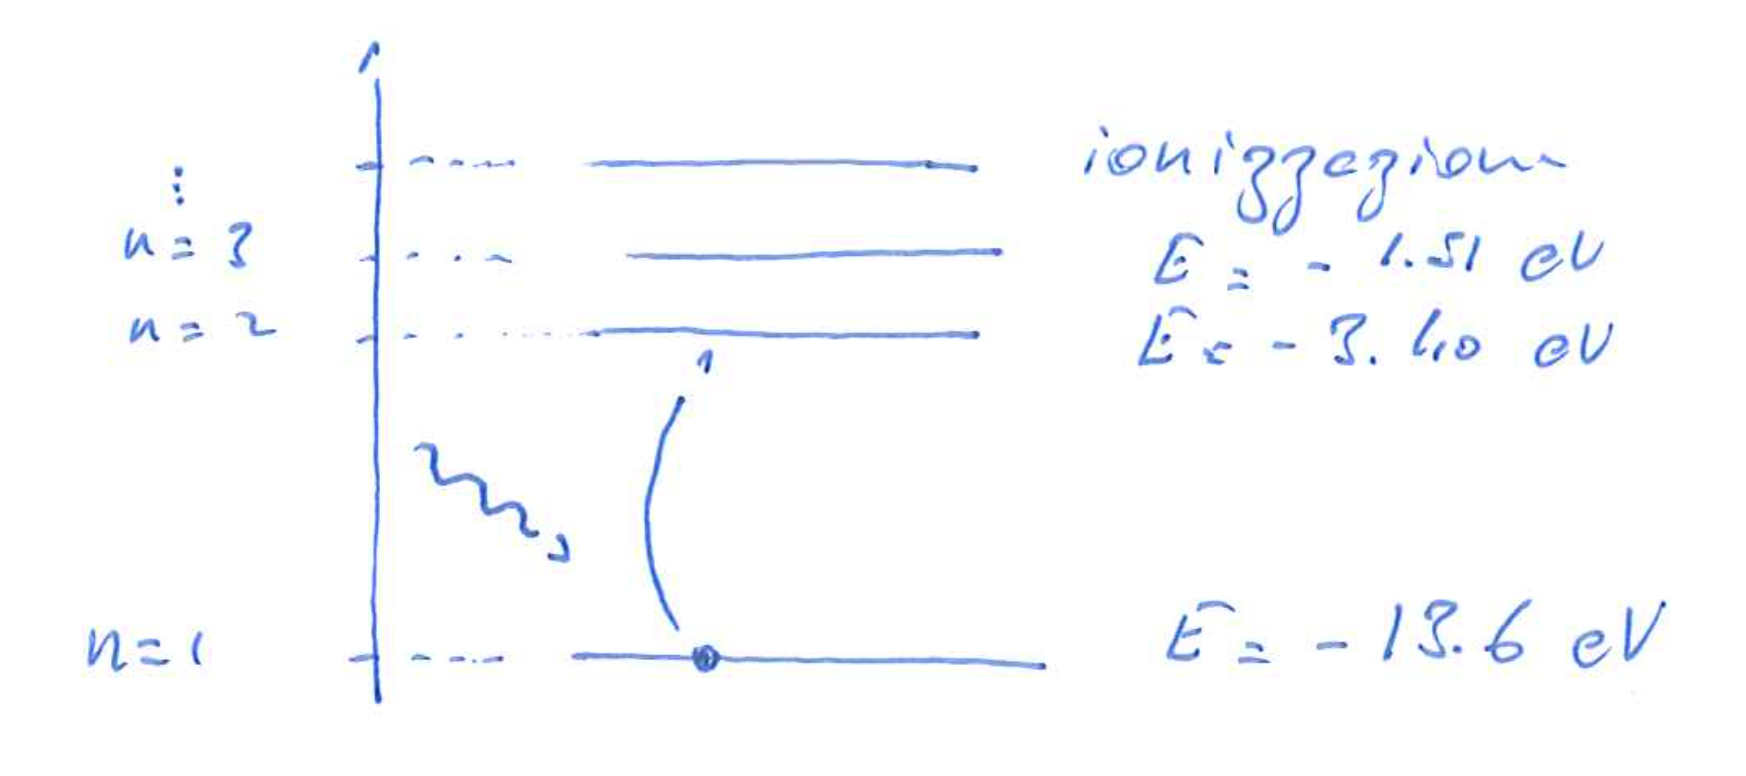
\includegraphics[width=0.8\textwidth]{Hydrogen}
\caption{Structure of the energy levels in an Hydrogen atom}  \label{fig:Hydrogen}
\end{figure}{}

In the case of the Hydrogen atom in its ground state, it should be noted that if energy is given to the system through a photon, with an energy that does not correspond to the difference with its first excited level, the received energy will be transformed only to motion of the hydrogen atom. It is therefore important to cover the widest possible range of energies to ensure that the system does not have an internal structure. \\

The concept of {\it elementary particle} is therefore not definitive and is strictly applicable only for a given range of energies. 
Another way to look at this, which is fundamental in these lectures, is through the quantum nature of microscopic particles and their duality with waves. One starts from the {\it de Broglie} hypothesis that matter particles have a wave-like nature with a wavelength related to their momentum:
$$ \lambda = \frac{h}{p}, $$
which is the generalisation of Einstein's interpretation of the photoelectric effect, whereby electrons can only receive energy in discrete quanta by photons with energy $E = h \nu$, related to the photon frequency $\nu$, and where $h$ is Planck's constant. \\

Heisenberg's uncertainty principle relies on a fundamental hypothesis: it postulates that measuring accurately the position would necessarily disturb the momentum, which could in turn not be measured accurately -- and vice versa:

$$ \Delta p \cdot \Delta x \geq \frac{\hslash}{2}$$

\noindent where $\hslash = h/2\pi$, and $\Delta$ represents the standard deviation of length $x$ and momentum $p$. This view is fundamental in the quantum mechanical interpretation of a particle as a wave. From this principle it is clear that, in order to resolve small distances, large momenta {\it "disturbances"} are needed, and therefore probes (like for example photons) with larger momenta of typically:

$$ p \geq \frac{h}{4\pi x}.$$

Using simple light probes (photons), optical microscopes can naturally resolve structures of the size of approximately \SI{0.2}{\micro\meter}. Electron microscopes (which use as probes electrons) can resolve atomic sizes with resolutions of \SI{0.05}{nm} via Tunnel Transmission Electron Microscopy (TEM). Another sophisticated technique is Scanning Tunneling Microscopy, which makes use of tunnelling electrons, by scanning the material with a conducting tip close to its surface, and applying an electric voltage between the two, thus allowing electrons to tunnel through the vacuum. The position will then be a function of the measured current and the resolution achievable is approximately \SI{0.1}{nm}. See Figure~\ref{fig:Microscope} for an illustration.

\begin{figure}
  \centering
  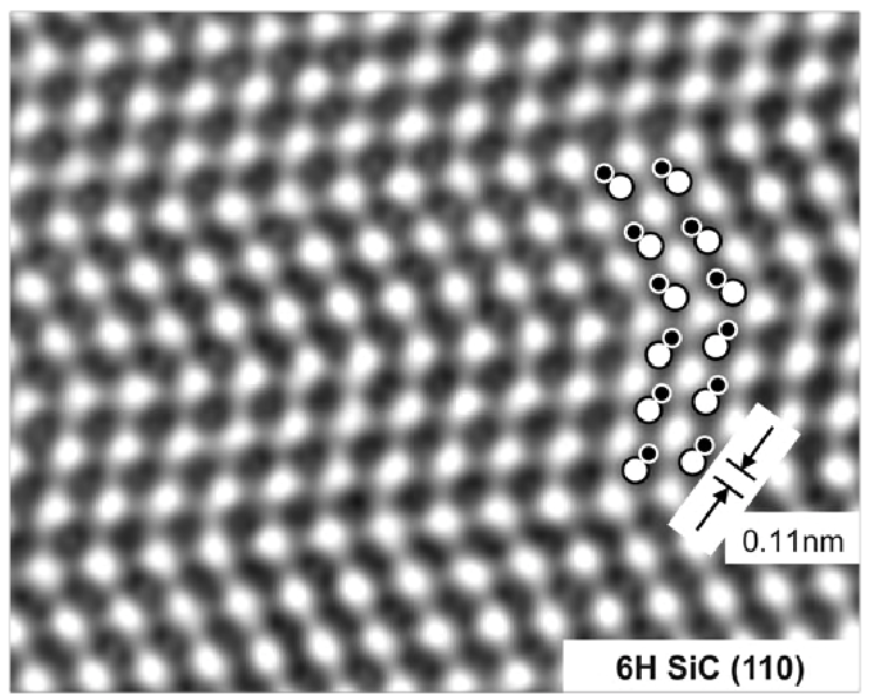
\includegraphics[width=0.4\textwidth]{Microscope-1}
  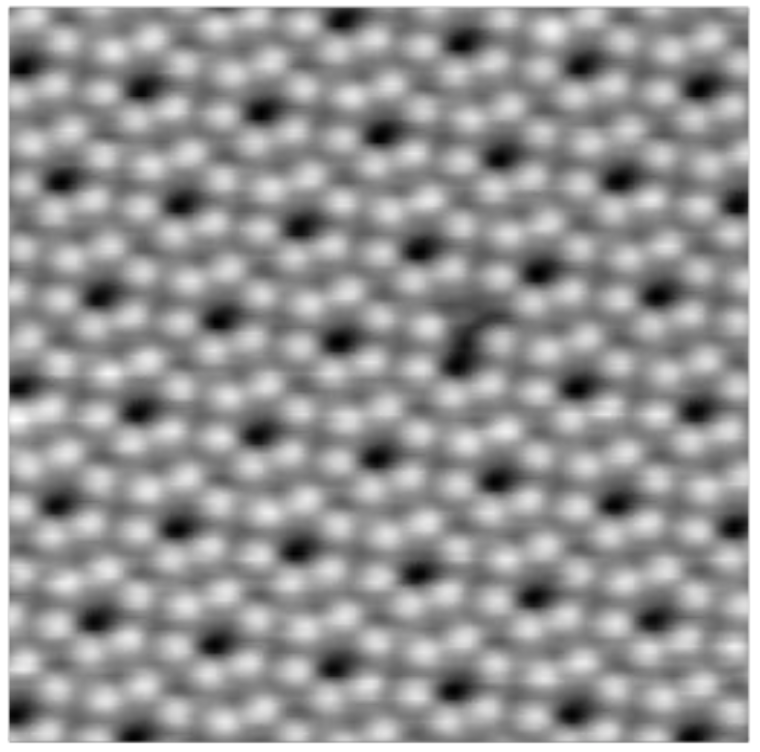
\includegraphics[width=0.4\textwidth]{Microscope-2}
\caption{Example image reconstructed via Scanning Tunneling Microscopy.}  \label{fig:Microscope}
\end{figure}{}

 Higher energies are needed to resolve even smaller distance scales, which requires new sources of particles at higher energies. As we will see in these lectures, a number of such sources have been used.  \\
 
  As will be discussed in Chapter~\ref{decaylaws-I}, the discovery of radioactivity provided sources of photons, electrons and $\alpha$ particles at higher energies (energies which nowadays would be deemed as fairly low!). Another very interesting source of high energy particles, as will be discussed in Chapter~\ref{}, are cosmic rays, which constitute the source of highest energy particles to date. Later, with the development of Nuclear, Subnuclear and Particle Physics came sources of particles at increasingly larger energies, reached through accelerators and eventually colliders. Accelerator techniques will be discussed in Chapter~\ref{accelerators}.

\section{Fundamental Forces}

In his first formulation of a Modern Physics theory of gravitation, Newton recognized immediately that there was a {\it "great absurdity"} in imagining that a force could be acting from one body to another at a distance! As he stated unambiguously in his letter to Bentley in 1692: 

\begin{quote}
    "It is inconceivable that inanimate Matter should, without the Mediation of something else, which is not material, operate upon, and affect other matter without mutual Contact...That Gravity should be innate, inherent and essential to Matter, so that one body may act upon another at a distance through a Vacuum, without the Mediation of any thing else, by and through which their Action and Force may be conveyed from one to another, is to me so great an Absurdity that I believe no Man who has in philosophical Matters a competent Faculty of thinking can ever fall into it. Gravity must be caused by an Agent acting constantly according to certain laws; but whether this Agent be material or immaterial, I have left to the Consideration of my readers."
\end{quote}

Another very important aspect that will be developed in these lectures is that of forces or interactions.

% Always give a unique label
% use \chaptermark{}
% to alter or adjust the chapter heading in the running head

\section*{Take-home lessons}
\begin{itemize}
    \item Modern Physics includes Nuclear and Subnuclear physics; Particle Physics is a branch of the latter, and studies the fundamental components and forces of the Universe.
    \item A particle is considered as elementary if it shows no internal structure, i.e. if one gives energy to that particle, this energy will be used only for the purpose of motion (kinetic energy).
    \item We consider a particle as elementary if no experiment to date has proved it isn't -- so the definition of elementary particle is somehow provisional.
    \item The Heisenberg uncertainty principle implies that, in order to probe smaller distances, we need higher energies.
    \item Radioactivity, accelerators, colliders and cosmic rays are sources of particles of higher and higher energy.
    \item Relativity and Quantum Mechanics are two necessary building blocks of our understanding of elementary particles.
    \item The Standard Model of particle physics is the model which best describes elementary particles and their interactions.
    \item Forces, or interactions, have a range: two bodies A and B cannot interact instantaneously, but they rather exchange particles which mediate that interaction.
\end{itemize}
\section*{Questions}
\begin{itemize}
    \item Let's suppose you have a billiard ball. How can you tell whether it's an elementary particle or not?
\end{itemize}


\begin{thebibliography}{99.}%
\bibitem{Popper:Scientificity} K. Popper, ``The Logic of Scientific Discovery''. Abingdon-on-Thames: Routledge. p. 66. (ISBN 0-41527843-0.)

\bibitem{Feynman:PhysicalLaws} R. Feynman, ``The Character of Physical Law''. Modern Library. ISBN 978-0-679-60127-2.
\end{thebibliography}
